 \documentclass{article}
\usepackage[top=2.5cm, bottom=2.5cm, left=2.5cm, right= 2.5cm]{geometry}

\usepackage[letterspace=60]{microtype} % Espaçamento entre as letras
\usepackage[utf8]{inputenc}
\usepackage{enumitem}
\usepackage{eurosym}
\usepackage{multirow} % Tabelas de formatação complexa
\usepackage{indentfirst} %Identar o primeiro parágrafo da seção
\usepackage[brazil]{babel} % Hifens e textos segundo as regras da língua portuguesa (Brasil)[e.g.: References -> Referências]
\usepackage{graphicx}
\usepackage{float}
\usepackage{ragged2e} % https://www.overleaf.com/learn/latex/Text_alignment
\usepackage{titlesec}
\setcounter{secnumdepth}{4}
\usepackage{amssymb}
\usepackage{graphicx}
\usepackage{blindtext}
\usepackage{pdfpages}
\usepackage{hyphenat}

\titleformat{\paragraph}
{\normalfont\normalsize\bfseries}{\theparagraph}{1em}{}
\titlespacing*{\paragraph}
{0pt}{3.25ex plus 1ex minus .2ex}{1.5ex plus .2ex}

% https://tex.stackexchange.com/questions/78842/nested-enumeration-numbering
\renewcommand{\labelenumii}{\theenumii}
\renewcommand{\theenumii}{\theenumi.\arabic{enumii}.}

\begin{document}
\newgeometry{top=4cm,left=3cm,right=3cm,bottom=4cm,heightrounded}
\begin{titlepage}
\centering
UNIVERSIDADE FEDERAL DE MINAS GERAIS \\
DEPARTAMENTO DE ENGENHARIA MECÂNICA\\
\vspace{\stretch{4}}
{\Large Metodologia para Cálculo Estrutural de \\
Motor de Foguete de Proelente Sólido \\}

\vspace{\stretch{1}}
Samuel Renan Costa Morais\\
\vspace{\stretch{4}}
Belo Horizonte\\ 2020

\end{titlepage}

\lsstyle % Espaçamento entre as letras
% \begin{hyphenrules}{nohyphenation} -- Inibe hifens


\newpage

\tableofcontents

\newpage

% Inclui o arquivo "01Objetivo.tex" existente neste projeto
\section{Resumo}


\section{Objetivo}
% Qual é o tema e sua relevância; 
\justifying
Desenvolver uma aplicação web com uma metodologia para dimensionamento de motores de foguete com propelente sólido até classe G permitindo a otimização considerando propriedades pré-definidas pelo usuário.

\section{Justificativa}


\section{Introdução}


\section{Revisão Bibliográfica}


\section{Metodologia}


\section{Discussão de Resultados}


\section{Conclusões}


\section{Referências Bibliográficas}


\section{Cronograma}
\justifying
Devido à pandemia e a consequente incerteza no calendário acadêmico da UFMG em 2020, o cronograma foi divido por semanas e sem datas específicas. Portanto, considerou-se que os 2 semestres que consistirão no desenvolvimento desse projeto terão, aproximadamente, 38 semanas.

As tarefas desse projeto foram dividas em três grupos: Desenvolvimento, Relatório e Modelagem. O grupo  Desenvolvimento engloba as atividades relacionadas à programação e modelagem de banco de dados. Relatório são aquelas atividades relacionadas ao desenvolvimento do relatório do projeto e modelagem é a pesquisa e definição da metodologia implementada.

    \begin{figure}[H]
    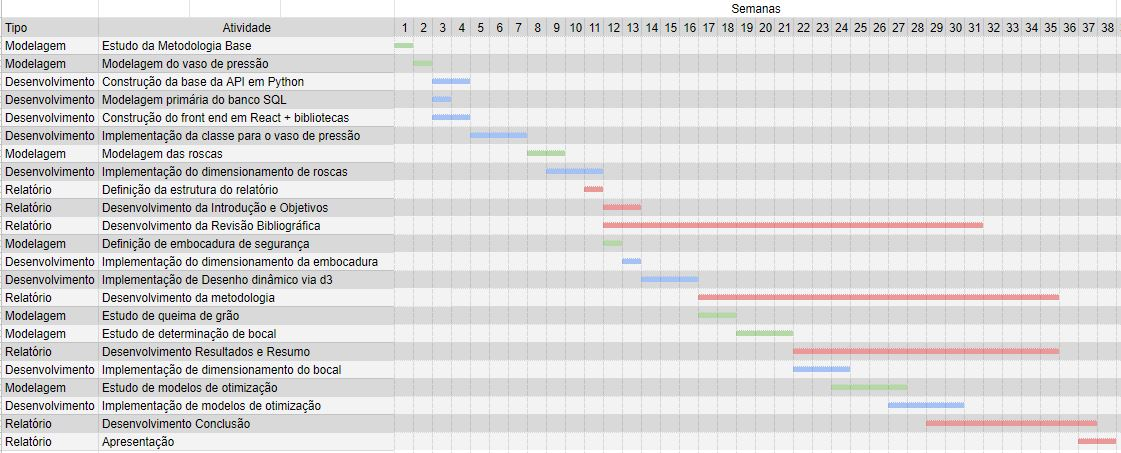
\includegraphics[scale=0.5]{Imagens/Cronograma.jpg}
    \centering
    \caption{Cronograma do Projeto}
    \label{Schedule}
    \end{figure}
%\end{hyphenrules}
\end{document}
